\section{Additional figures}\label{app:A}

\begin{figure}[H]
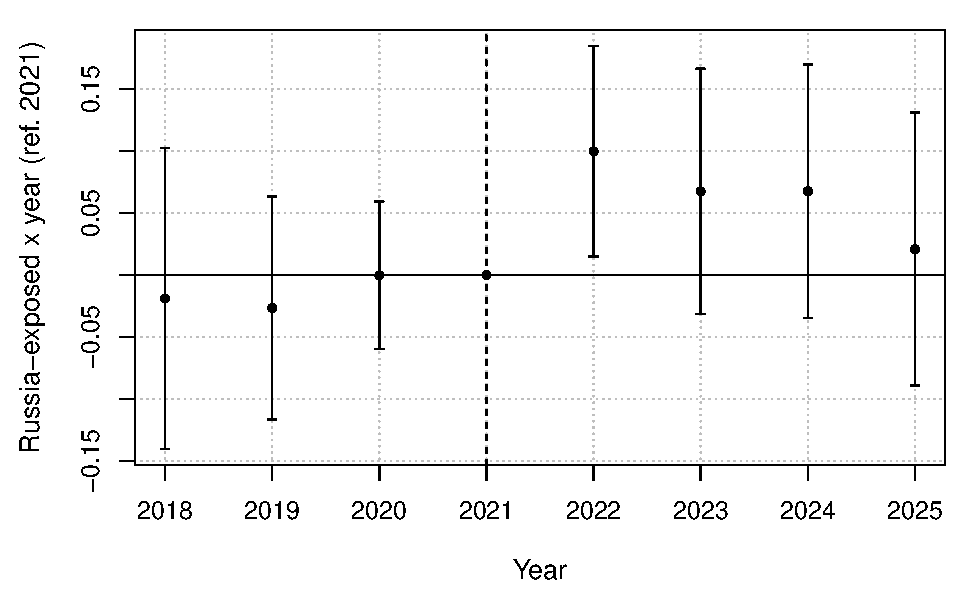
\includegraphics[width=\textwidth]{figures/figA1_firststage_annual.pdf}
\caption{The first stage, receiving a remittance, Russia-exposed and other destinations}
\label{fig:A1}
\begin{figurenotes}
The figure shows the coefficients of the interaction of Russia exposure with each calendar year, relative to 2021, from a regression of receiving a remittance on household and year fixed effects. The sample covers only the baseline migrant households, 254 households (204 Russia-exposed, 50 in other destinations), 18,802 household round observations over 82 survey rounds, September 2018 to June 2025. The vertical lines show the 95 percent confidence intervals, and the standard errors are clustered at the household level. The dashed vertical line marks the February 2022 invasion. Source. The author's calculations from L2CU.
\end{figurenotes}
\end{figure}

\begin{figure}[H]
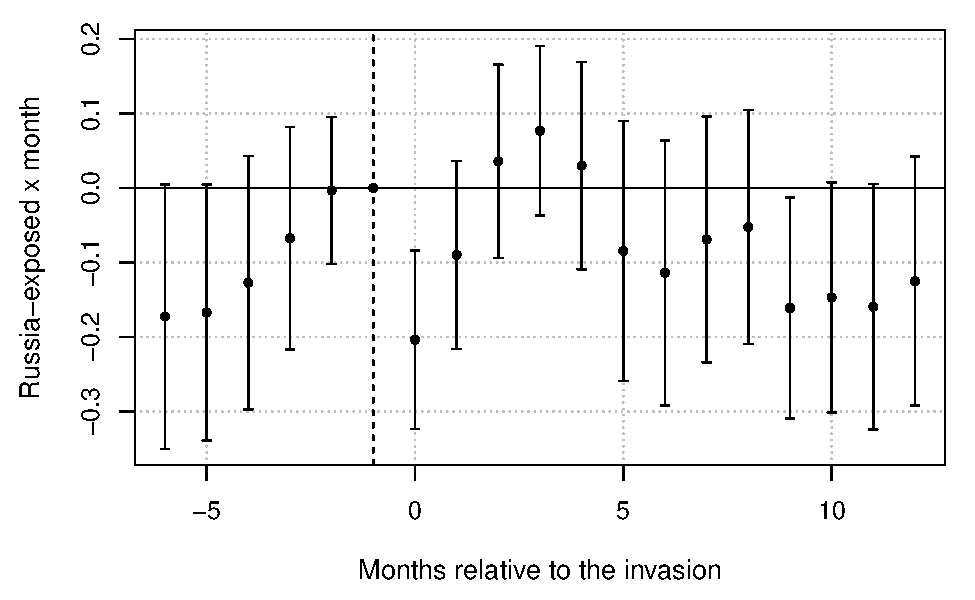
\includegraphics[width=\textwidth]{figures/figA2_firststage_monthly.pdf}
\caption{The first stage, receiving a remittance, monthly event study}
\label{fig:A2}
\begin{figurenotes}
The figure shows the coefficients of the interaction of baseline Russia exposure with each survey round in event time, relative to the round immediately preceding the invasion, from a regression of receiving a remittance on household and survey round fixed effects. The outcome is de-seasonalized as described in Section~\ref{sec:6-6}. The sample covers the baseline migrant households, 254 households (204 Russia-exposed, 50 in other destinations). The vertical lines show the 95 percent confidence intervals, and the standard errors are clustered at the household level. The dashed vertical line marks the invasion. Source. The author's calculations from L2CU.
\end{figurenotes}
\end{figure}

\begin{figure}[H]
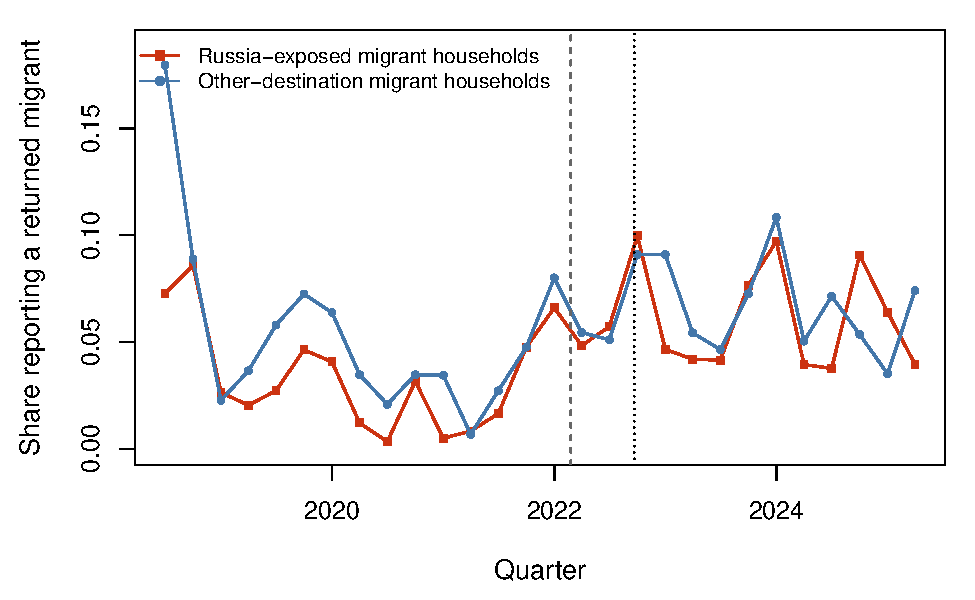
\includegraphics[width=\textwidth]{figures/figA3_return_migration.pdf}
\caption{Reported return migration, by quarter}
\label{fig:A3}
\begin{figurenotes}
The figure shows the raw share of households reporting that a member had returned from abroad, by calendar quarter, separately for baseline Russia-exposed and other destination migrant households. No controls or adjustments are applied. The dashed vertical line marks the February 2022 invasion and the dotted vertical line the partial military mobilization announced on 21 September 2022. The series covers 82 survey rounds, September 2018 to June 2025. Source. The author's calculations from L2CU.
\end{figurenotes}
\end{figure}

\begin{figure}[H]
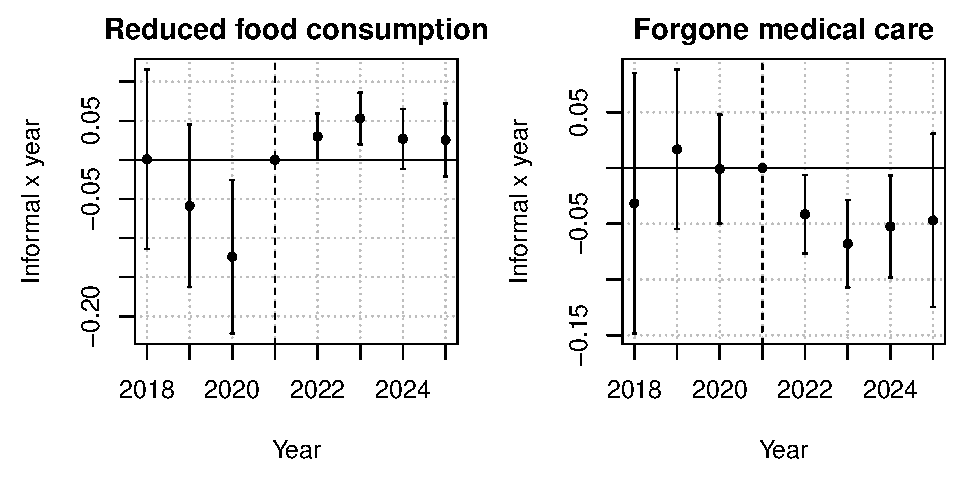
\includegraphics[width=\textwidth]{figures/figA4_secondary.pdf}
\caption{Secondary outcomes, annual event studies}
\label{fig:A4}
\begin{figurenotes}
Each panel shows the coefficients of the interaction of the baseline informality indicator with each calendar year, relative to the 2021 reference year, from a regression of the outcome on household and year fixed effects. The sample covers 190 Russia migrant households and 14,128 household round observations over 82 survey rounds, September 2018 to June 2025. The vertical lines show the 95 percent confidence intervals, and the standard errors are clustered at the household level. The dashed vertical line marks the February 2022 invasion. Source. The author's calculations from L2CU.
\end{figurenotes}
\end{figure}

\begin{figure}[H]
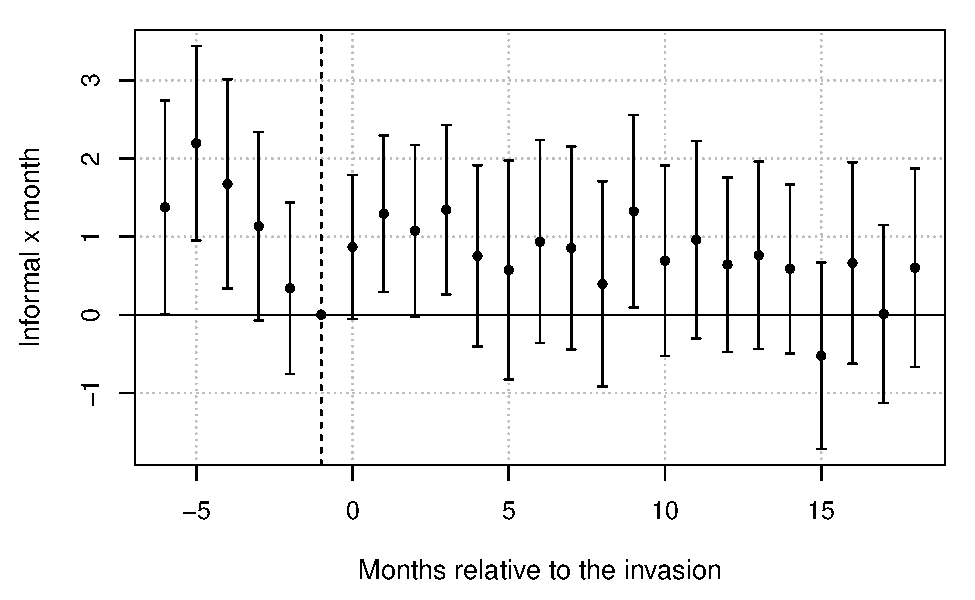
\includegraphics[width=\textwidth]{figures/figA5_income_channel.pdf}
\caption{Remittance value, monthly event study}
\label{fig:A5}
\begin{figurenotes}
The figure shows the coefficients of the interaction of the baseline informality indicator with each survey round in event time, relative to the round immediately preceding the invasion, from a regression of the de-seasonalized inverse hyperbolic sine of the remittance amount in US dollars on household and survey round fixed effects. Amounts are converted at the fixed rates reported in Table~\ref{tab:C3} and winsorized at the 99th percentile. The sample covers 190 Russia migrant households, 14,128 household round observations. The standard errors are clustered at the household level. The coefficients are measured against the single round before the invasion, while the pooled estimate in Table~\ref{tab:B5} differences the whole pre-shock period against the whole post-shock period, so the two are not comparable in level. Source. The author's calculations from L2CU.
\end{figurenotes}
\end{figure}

\clearpage
\section{Additional tables}\label{app:B}

This appendix reports the raw outcome means before and after the invasion, the welfare outcomes with the multiple testing correction, the links of the income chain and their decomposition by phase, the aggregate comparison between Russia-exposed and other migrant households, a comparison of designs in the closest literature, and then the robustness of the main estimate to the baseline assignment window, the full annual interaction coefficients, the alternative definitions of informality and the heterogeneity by baseline remittance dependence.


\begin{table}[H]
\caption{Outcome means before and after the invasion, by baseline migrant employment formality}
\label{tab:B10}
\footnotesize
\begin{tblr}[booktabs]{width=\textwidth, colsep=3pt, colspec={X[l]rrrrrrr}}
Outcome & Informal, pre & Informal, post & Change & Formal, pre & Formal, post & Change & Difference \\
\midrule
Food insecurity & 0.076 & 0.308 & +0.232 & 0.097 & 0.069 & $-$0.028 & +0.260 \\
Reduced food consumption & 0.096 & 0.012 & $-$0.083 & 0.215 & 0.030 & $-$0.185 & +0.102 \\
Forgone medical care & 0.202 & 0.135 & $-$0.067 & 0.123 & 0.084 & $-$0.039 & $-$0.028 \\
\end{tblr}
\begin{tablenotes}
The table gives the unadjusted household round means of each binary outcome. The pre-shock period covers rounds 1 to 42 (September 2018 to February 2022) and the post-shock period covers rounds 43 to 82 (March 2022 to June 2025). The sample is the Russia migrant households classified by the majority rule over baseline employment formality, with ties excluded, 53 informal and 137 formal households, 14,128 household round observations, of which 7,491 before the invasion and 6,637 after. Change is the within-group change, the post-shock mean minus the pre-shock mean. Difference is the change in the informal households minus the change in the formal households, that is the unadjusted difference-in-differences. No weights, control variables or fixed effects are applied. Source. The author's calculations from the L2CU household and individual files.
\end{tablenotes}
\end{table}

\begin{table}[H]
\caption{Welfare outcomes, with the Romano and Wolf multiple testing correction}
\label{tab:B9}
\footnotesize
\begin{tblr}[booktabs]{width=\textwidth, colsep=3pt, colspec={X[1.1,l]rrrrX[1.3,r]}}
Outcome & Coefficient & Clustered SE & Romano-Wolf p & Pre-trend p & Verdict \\
\midrule
Food insecurity & +0.279 & (0.042) & 0.000 & 0.55 & Passes both gates \\
Reduced food consumption & +0.085 & (0.031) & 0.024 & 0.09 & Driven by the pre-shock period \\
Forgone medical care & $-$0.052 & (0.018) & 0.017 & 0.68 & Passes both gates, negative \\
Inability to pay utilities & +0.002 & (0.017) & 0.918 & --- & Null \\
Water disruption (placebo) & $-$0.027 & (0.017) & 0.196 & --- & Placebo clean \\
Distress coping (composite) & $-$0.081 & (0.018) & 0.002 & 0.010 & Fails pre-trend, excluded \\
\end{tblr}
\begin{tablenotes}
Each row reports the Informal $\times$ Post coefficient from a separate regression of the outcome on household and survey round fixed effects, 190 households, 14,128 household round observations, 82 rounds, September 2018 to June 2025. The food and medical outcomes are de-seasonalized as described in Section~\ref{sec:6-6}; the utility and water outcomes enter unadjusted. The Romano and Wolf p-values control the familywise error rate across the six outcomes listed here and are computed by randomization inference with 2,000 permutations of the baseline informality label across households and a fixed seed, so they are reproducible from the replication script but would shift slightly under a different draw. The Romano-Wolf procedure uses pooled calendar-month means for the adjustment, so the t-statistics reported here differ slightly from the coefficient-to-standard-error ratios in the preceding columns. The pre-trend p-values test the joint significance of the eleven pre-invasion event time interactions and are shown only for outcomes that pass the multiple testing correction. The standard errors are clustered at the household level. The composite coping indicator passes the correction but fails the pre-shock trend test and is excluded on identification grounds rather than on significance. Source. The author's calculations from L2CU.
\end{tablenotes}
\end{table}

\begin{table}[H]
\caption{The mechanism, the income chain, informal and formal households}
\label{tab:B5}
\begin{tblr}[booktabs]{width=\textwidth, colspec={lrrr}}
Link & Coefficient & Clustered SE & Pre-trend p \\
\midrule
Migrant employed abroad & $-$0.099 & (0.061) & 0.10 \\
Migrant still abroad & $-$0.077 & (0.065) & 0.23 \\
Migrant sends remittances & $-$0.060 & (0.044) & 0.09 \\
Remittance value (inverse hyperbolic sine, USD) & $-$0.390 & (0.285) & 0.10 \\
Composite: income channel intact & $-$0.073* & (0.041) & 0.08 \\
\end{tblr}
\begin{tablenotes}
Each row reports the Informal $\times$ Post coefficient from a separate regression of the de-seasonalized outcome on household and survey round fixed effects, 190 households, 14,128 household round observations, 82 rounds, September 2018 to June 2025. The composite income channel indicator equals one when the migrant both works abroad and sent money in the last 30 days, and its two sided p-value is 0.075, while the one sided p-value under the directional hypothesis that informal households lose income is 0.038. The standard errors are clustered at the household level. The pre-trend p-values test the joint significance of the eleven pre-invasion event time interactions. (* significant at the 10 percent level.) Source. The author's calculations from L2CU.
\end{tablenotes}
\end{table}

\begin{table}[H]
\caption{The aggregate effect on migrant households, Russia-exposed and other destinations}
\label{tab:B6}
\begin{tblr}[booktabs]{width=\textwidth, colspec={lrrrr}}
Outcome & Russia-exposed $\times$ Post & Clustered SE & p-value & Pre-trend p \\
\midrule
Food insecurity & +0.027 & (0.026) & 0.30 & 0.556 \\
Reduced food consumption & $-$0.045 & (0.034) & 0.18 & 0.303 \\
Forgone medical care & +0.020 & (0.019) & 0.31 & 0.216 \\
\end{tblr}
\begin{tablenotes}
Each row reports the Russia-exposed $\times$ Post coefficient from a regression of the de-seasonalized outcome on household and survey round fixed effects, following specification~\eqref{eq:did} with the Russia exposure indicator in place of the informality indicator. The sample covers all baseline migrant households, 254 households, of which 204 are Russia-exposed and 50 have migrants in other countries, 18,802 household round observations over 82 rounds, September 2018 to June 2025. The standard errors in parentheses are clustered at the household level. The pre-trend p-values test the joint significance of the eleven pre-invasion event time interactions. Source. The author's calculations from L2CU.
\end{tablenotes}
\end{table}


\begin{table}[H]
\caption{The mechanism by phase, the income channel intact}
\label{tab:B8}
\begin{tblr}[booktabs]{width=\textwidth, colspec={lrrr}}
Phase & Coefficient & Clustered SE & p-value \\
\midrule
Invasion (Mar--Sep 2022) & $-$0.032 & (0.044) & 0.47 \\
Mobilization (Oct 2022--Mar 2023) & $-$0.059 & (0.053) & 0.27 \\
Apr--Sep 2023 & $-$0.125** & (0.051) & 0.014 \\
Oct 2023 onwards & $-$0.078* & (0.046) & 0.089 \\
\end{tblr}
\begin{tablenotes}
The table reports the coefficients of the interaction of the baseline informality indicator with each post-invasion phase, from a single regression of the de-seasonalized income channel composite on household and survey round fixed effects, 190 households, 14,128 household round observations, 82 rounds, September 2018 to June 2025. The phases follow the sequence described in Section~\ref{sec:3-3}. The standard errors in parentheses are clustered at the household level. (** significant at the 5 percent level, * at 10 percent.) Source. The author's calculations from L2CU.
\end{tablenotes}
\end{table}

\begin{table}[H]
\caption{Robustness to the baseline assignment window}
\label{tab:B1}
\begin{tblr}[booktabs]{width=\textwidth, colspec={lrrrr}}
Baseline window & Informal & Formal & Informal $\times$ Post & Pre-trend p \\
\midrule
Rounds 39--42 (main, 4 rounds) & 53 & 137 & +0.279*** (0.042) & 0.55 \\
Rounds 37--42 (6 rounds) & 65 & 152 & +0.252*** (0.038) & 0.73 \\
Rounds 34--42 (9 rounds) & 72 & 154 & +0.270*** (0.036) & 0.69 \\
Rounds 31--42 (12 rounds) & 79 & 153 & +0.265*** (0.036) & 0.65 \\
Rounds 25--42 (18 rounds) & 85 & 168 & +0.253*** (0.034) & 0.73 \\
Rounds 21--42 (22 rounds) & 89 & 172 & +0.255*** (0.035) & 0.55 \\
\end{tblr}
\begin{tablenotes}
Each row reports the coefficient on Informal $\times$ Post from the de-seasonalized specification~\eqref{eq:did}, with both treatment and control groups reassigned using the indicated baseline window. All windows end at round 42, the last pre-invasion round. Widening the window enlarges the sample, because a household whose migrants are not observed in rounds 39 to 42 may be observed in an earlier round: the number of Russia migrant households rises from 204 in the four-round window to 226, 237, 244, 269 and 272 as the window is extended, so the group sizes reported here are not bounded by the 204 of the main specification. Standard errors, in parentheses, are clustered at the household level. Pre-trend p-values test the joint significance of eleven pre-invasion event-time interactions. Sample period: 82 survey rounds, September 2018 to June 2025. The main specification retains the four-round window because it gives the tightest temporal link between the measured status and the migrant's situation at the shock. (***: significant at the 1 percent level.) Source: author's calculations from L2CU.
\end{tablenotes}
\end{table}

\begin{table}[H]
\caption{Annual interaction coefficients, food insecurity}
\label{tab:B2}
\begin{tblr}[booktabs]{width=\textwidth, colspec={lrr}}
Year & Informal $\times$ year & Clustered SE \\
\midrule
2018 & +0.067** & (0.032) \\
2019 & +0.028 & (0.024) \\
2020 & $-$0.002 & (0.024) \\
2021 & reference & --- \\
2022 & +0.301*** & (0.043) \\
2023 & +0.426*** & (0.062) \\
2024 & +0.190*** & (0.033) \\
2025 & +0.083** & (0.036) \\
\end{tblr}
\begin{tablenotes}
The table reports the coefficients plotted in Figure 2, from a regression of food insecurity on the interaction of the baseline informality indicator with each calendar year, with household and year fixed effects, 2021 omitted as the reference year. The sample covers 190 Russia migrant households and 14,128 household round observations over 82 survey rounds, September 2018 to June 2025. The standard errors in parentheses are clustered at the household level. (*** significant at the 1 percent level, ** at 5 percent, * at 10 percent.) Source. The author's calculations from L2CU.
\end{tablenotes}
\end{table}

\begin{table}[H]
\caption{Alternative definitions of informality}
\label{tab:B3}
\footnotesize
\begin{tblr}[booktabs]{width=\textwidth, colspec={lrrrrr}}
Definition & Informal & Formal & Informal $\times$ Post & Pre-trend p & Observations \\
\midrule
Majority rule (main specification) & 53 & 137 & +0.279*** (0.042) & 0.55 & 14,128 \\
Any informal migrant at baseline & 85 & 117 & +0.219*** (0.032) & 0.68 & 15,026 \\
All baseline migrants informal & 40 & 117 & +0.213*** (0.046) & 0.50 & 11,678 \\
\end{tblr}
\begin{tablenotes}
Each row reports the Informal $\times$ Post coefficient from the de-seasonalized specification~\eqref{eq:did} on household and survey round fixed effects, with the treatment indicator defined by the stated rule within the 202 baseline Russia migrant households that return a usable formality response. The formal group is defined identically under the last two rules, as households with no informal migrant, which is why the count of 117 is the same in both; under the third rule the mixed households are dropped, so the two groups sum to 157 rather than 202. The standard errors in parentheses are clustered at the household level. The pre-trend p-values test the joint significance of the eleven pre-invasion event time interactions. Sample period 82 survey rounds, September 2018 to June 2025. (*** significant at the 1 percent level.) Source. The author's calculations from L2CU.
\end{tablenotes}
\end{table}

\begin{table}[H]
\caption{Heterogeneity by baseline remittance dependence}
\label{tab:B4}
\begin{tblr}[booktabs]{width=\textwidth, colspec={lrrrr}}
Subsample & Informal & Formal & Informal $\times$ Post & Observations \\
\midrule
Above median dependence & 15 & 49 & +0.467*** (0.064) & 4,801 \\
At or below median dependence & 38 & 88 & +0.205*** (0.045) & 9,327 \\
\end{tblr}
\begin{tablenotes}
The table splits the estimation sample at the median share of baseline months in which the household received a remittance (median 0.50) and reports the Informal $\times$ Post coefficient from the de-seasonalized specification~\eqref{eq:did} with household and survey round fixed effects within each subsample. The standard errors in parentheses are clustered at the household level. Sample period 82 survey rounds, September 2018 to June 2025. The subsamples are small and the split is presented as descriptive rather than as an identified heterogeneity test. (*** significant at the 1 percent level.) Source. The author's calculations from L2CU.
\end{tablenotes}
\end{table}

% The rotated float is placed last in Appendix B so that its number and its
% physical position agree. A sidewaystable declared mid-sequence is numbered
% where it is declared but deferred to a float page, printing out of order.
\begin{sidewaystable}[htbp]
\caption{A comparison of designs in the closest literature}
\label{tab:B7}
\footnotesize
\begin{tblr}[booktabs]{rowsep=2pt, width=\textwidth, colspec={X[.7]X[.8]X[1.1]X[.9]X[1.5]}}
Study & Setting & Source of variation & Outcome & Principal finding \\
\midrule
Yang (2006) & Philippines, Asian crisis & Destination exchange-rate movements & Return migration & Destination shocks shape return decisions \\
Yang and Choi (2007) & Philippines & Rainfall shocks as IV for household income & Remittances, consumption & \textasciitilde{}60\% of income declines replaced; consumption insured in migrant households \\
Yang (2008) & Philippines, Asian crisis & Destination exchange-rate movements & Remittances, schooling, enterprise & Elasticity 0.60; positive shocks raise human capital and entrepreneurship \\
Shimizutani and Yamada (2021) & Tajikistan, COVID-19 & Migrant vs. non-migrant households, monthly panel & Household welfare battery & Effects sharp but transitory; migrant households more resilient \\
Bossavie, Ozden, Rude and Zhou (2025) & Kyrgyz Republic, 2022 Russia shock & Difference-in-differences, high-frequency panel & Migration flows, composition & Male migration fell, female rose; compositional shift among migrants \\
Amuedo-Dorantes and Bansak (2011) & United States, IRCA & Legalized vs. already-legal population & Employment, wages & Employment fell, wage growth rose after legalization \\
Elias, Monras and V\'azquez-Grenno (2025) & Spain & Work-permit grants and regularization & Wages, employment & Regularization raises wages by reducing employer market power \\
This thesis & Uzbekistan, 2022 Russia shock & 2022 Russia shock interacted with baseline employment formality, DiD & Food insecurity, welfare battery & Aggregate effect near zero; informal-migrant households +28 pp relative to formal-migrant households \\
\end{tblr}
\begin{tablenotes}
The table compares the identification strategy and the main result of the studies closest to this analysis. IV means instrumental variables. The last row summarizes the design and the result of this thesis for comparison. Source. Compiled by the author from the cited studies.
\end{tablenotes}
\end{sidewaystable}

\clearpage
\section{Variable definitions and sample construction}\label{app:C}

\subsection*{Comparisons considered and rejected}

Two candidate designs discussed in Section~\ref{sec:6-1} were rejected on predetermined checks, and each is recorded here because it clarifies what the main comparison can and cannot identify.

The first compared Russia migrant households with households that had no migrant at all. Households without a migrant receive almost no remittances, so their remittance line is flat at zero, while in migrant households the receipt of transfers moves with the seasons, employment conditions and transfer channels. It is not credible that two groups with fundamentally different outcome processes satisfy the parallel trends condition, and the first stage pre-shock trend test rejects the assumption. More importantly, a control group that cannot experience the outcome is not a counterfactual for a group that can.

The second split households by their pre-shock dependence on remittances and compared active receivers with non-receivers. This gave very large first stage falls of more than 30 percentage points, but the comparison is mechanically distorted. Households selected into the treatment group because they receive a transfer in the baseline can mostly move only down, while those selected into the control group because they do not can mostly move only up, so part of the measured effect reflects regression to the mean created by the selection rule itself rather than the shock.

\subsection*{Agreement among baseline migrant records}

The majority rule of Section~\ref{sec:5-3} pools over two dimensions. A quarter of the households, 51 of the 202 Russia migrant households that return a usable formality answer, contribute records for more than one distinct migrant over the four baseline rounds, so their records can disagree with each other. Counted within a single round the figure is 49. The 202 households contribute 786 migrant records in total, an average of 1.29 per household-round in which at least one usable record is returned. This is higher than the 0.97 and 1.04 migrants abroad reported in Table~\ref{tab:1}, because that row divides a household's baseline migrant records by every baseline round in which the household is observed, including rounds that return no migrant record, while the figure here counts only the household-rounds that carry a usable formality record for a migrant in Russia. More often the rule resolves variation over time for a single migrant, who is observed in up to four rounds and whose reported status is not always the same in each. Records agree completely in 157 of the 202 households; of the 45 where they do not, 44 contain a migrant whose status changes between rounds and only 13 contain two migrants reporting different statuses. The same holds for the 12 tied households that are dropped, 9 of which are single migrant households whose reported status varies across the four rounds.

\begin{table}[H]
\caption{Variable definitions and survey wording}
\label{tab:C1}
\footnotesize
\begin{tblr}[booktabs]{rowsep=2pt, width=\textwidth, colspec={X[.75]X[1.9]X[.85]}}
Variable & Survey question & Coding \\
\midrule
Food insecurity & Was your household able to buy enough food for members for the past 30 days? & 1 if the answer is no \\
Reduced food consumption & Has your household reduced consumption of food over the past 30 days to pay for basic needs? & 1 if yes \\
Forgone medical care & In the last 30 days has it been necessary, for any reason, for any household member to give up medical care? & 1 if yes \\
Inability to pay utilities & Was your household financially unable to pay for utilities for the past 30 days? & 1 if yes \\
Water disruption (placebo) & Did you have any unexpected disruption in your water supply at home over the past 30 days? & 1 if yes \\
Distress coping (composite) & Did your household borrow money / take from savings / sell assets over the last 30 days to pay for basic needs? & 1 if any of the three is yes \\
Migrant destination & In what country is the migrant currently living? & Russia if the country is the Russian Federation \\
Migrant working abroad & Is the migrant currently working? & 1 if yes \\
Employment formality (treatment) & Is the migrant working abroad officially? & 1 informal if no, 0 formal if yes; do not know excluded \\
Migrant sends remittances & Did the migrant send any money to the household over the past month? & 1 if yes \\
Household receives remittances & Does your household receive any money from abroad from individuals who are not household members? & 1 if yes \\
\end{tblr}
\begin{tablenotes}
The table reports the survey wording of each variable used in the analysis and the coding applied. Household level outcomes are taken from the household file, migrant level variables from the individual file and aggregated to the household round level as the maximum across migrants. Source. The author's calculations from L2CU.
\end{tablenotes}
\end{table}

\begin{table}[H]
\caption{Sample construction}
\label{tab:C2}
\begin{tblr}[booktabs]{width=\textwidth, colspec={lr}}
Step & Households \\
\midrule
Households in the L2CU panel & 2,499 \\
With a migrant abroad in the baseline window (rounds 39 to 42) & 254 \\
of which migrants mostly in Russia & 204 \\
of which migrants mostly in other destinations & 50 \\
Without a migrant in the baseline window & 2,245 \\
Russia migrant households with a usable formality status & 190 \\
classified informal (majority rule) & 53 \\
classified formal (majority rule) & 137 \\
excluded (12 ties, 2 without a usable response) & 14 \\
\end{tblr}
\begin{tablenotes}
The table reports the construction of the estimation sample from the full panel. Baseline status is assigned over survey rounds 39 to 42, the four months preceding the invasion, and held fixed thereafter. Households whose baseline Russia migrants are evenly split between formal and informal work, and those for whom the formality question returns only do not know, are excluded. The resulting estimation sample contains 190 households and 14,128 household round observations. Source. The author's calculations from L2CU.
\end{tablenotes}
\end{table}

\begin{table}[H]
\caption{Currency conversion rates}
\label{tab:C3}
\begin{tblr}[booktabs]{width=\textwidth, colspec={lr}}
Currency & Units per US dollar \\
\midrule
Uzbek sum & 11,500 \\
US dollar & 1 \\
Russian ruble & 85 \\
Kazakh tenge & 460 \\
Euro & 0.91 \\
\end{tblr}
\begin{tablenotes}
Remittance amounts are reported in the currency selected by the respondent and converted to US dollars at the fixed period average rates above. About 84 percent of transfers in the panel are reported in US dollars, so the conversion affects a minority of observations. Fixed rather than time varying rates are used so that the converted series reflects the amount sent rather than exchange rate movements over the period. The currency in which a transfer is reported also changed after the invasion, and fixed rates do not remove this compositional change, which is a further reason why Section~\ref{sec:3-4} treats the extensive margin as the more reliable measure of the disruption. Source. The author's calculations from L2CU.
\end{tablenotes}
\end{table}